\documentclass{beamer}

\usepackage{beamerthemebars}
\usepackage{amsmath, amssymb}
\usepackage{ngerman,url}
\usepackage{algorithm2e}
\usepackage{graphicx}
\usepackage{wrapfig}
\usepackage[font={small}]{caption}

\setbeamertemplate{footline}[frame number]
\setbeamertemplate{caption}{\raggedright\insertcaption\par}

\begin{document}

\title{Parallele Numerik - Aufgabe 1}
\author{Rebecca Seelos, Alexander Lüngen, Joshua}

\frame{
  \titlepage
}

\section{Aufgabe 1}
\frame{
	\frametitle{Aufgabe 1 - Teil a}
	Die Reihenfolge in welcher die IDs der Threads ausgegeben werden ist jedes Mal unterschiedlich und ist auch nicht vorherzusagen.
}
\frame{
	\frametitle{Aufgabe 1 - Teil b}
	  \begin{tabular}{|l|l|r|r|r|}
	  		\hline
	  	- & Number of Threads & N & Time (s) & Speedup \\
	  	\hline
	  	sequential & 1 & 1000 & 0.002 & - \\
	  	& 1 & $10^{7}$ & 0.239 & - \\
	  	& 1 & $10^{8}$ & 2.388 & - \\
	  	& 1 & $10^{9}$ & 23.642 & - \\
	  	& 1 & $10^{10}$ & 239.508 & - \\
	  	\hline
	  	manual & 2 & 1000 & 0.002 & 1 \\
	  	& 2 & $10^{7}$ & 0.634 & - \\
	  	& 2 & $10^{8}$ & 6.461 & - \\
	  	& 2 & $10^{9}$ & 52.989 & - \\
	  	& 4 & $10^{9}$ & $\sim$ 120 & - \\
	  	\hline
	  \end{tabular}
}

\frame{
	\frametitle{Aufgabe 1 - Teil b}
	\begin{tabular}{|l|l|r|r|r|}
		\hline
		- & Number of Threads & N & Time (s) & Speedup \\
		\hline
		sequential & 1 & 1000 & 0.002 & - \\
		& 1 & $10^{7}$ & 0.239 & - \\
		& 1 & $10^{8}$ & 2.388 & - \\
		& 1 & $10^{9}$ & 23.642 & - \\
		& 1 & $10^{10}$ & 239.508 & - \\
		\hline
		reduction & 2 & $10^{7}$ & 0.121 & 1.9 \\
		& 2 & $10^{10}$ & 118.204 & 2 \\
		& 4 & $10^{7}$ & 0.062 & 3.9 \\
		& 4 & $10^{10}$ & 59.183 & 4 \\
		& 8 & $10^{10}$ & 29.689 & 8.0 \\
		& 16 & $10^{10}$ & 29.674 & 8.1\\
		& 32 & $10^{10}$ & 29.551 & 8.1 \\	
		\hline
	\end{tabular}
}

\frame{
	\frametitle{Aufgabe 1 - Teil c}
	\begin{tabular}{|l|l|r|r|r|}
		\hline 
		 Aufl"osung N & No. Threads &  Time (s) & Speedup \\
		\hline
		1000& 1 &  4.411 & - \\
		1000& 2 &  2.228 & 1.980 \\
		1000& 4 &  1.122 & 3.931 \\
		1000& 8 &  0.563 & 7.835\\
		1000& 16 &  0.567 & 7.780 \\
		\hline
		2000& 1 & 17.625 & - \\
		2000& 2 &  8.896& 1.981 \\
		2000& 4 &  4.493& 3.923 \\
		2000& 8 &  2.254& 7.819 \\
		2000& 16 &  2.248& 7.840 \\
		\hline
	\end{tabular}
}

\frame{
	\frametitle{Aufgabe 1 - Teil c}
	\begin{tabular}{|l|l|r|r|r|}
		\hline 
		Aufl"osung N & No. Threads &  Time (s) & Speedup \\
			\hline
		4000& 1 & 71.761 & - \\
		4000& 2 &  35.559 & 2.010 \\
		4000& 4 &  17.952& 3.997 \\
		4000& 8 &  8.978 & 7.991\\
		4000& 16 &  8.980 & 7.991 \\
		\hline
		5000& 1 &  110.143 & - \\
		5000& 2 &  55.564 & 1.982 \\
		5000& 4 &  27.951 & 3.94 \\
		5000& 8 &  13.995 & 7.870 \\
		5000& 16 &  14.020 & 7.856\\
		\hline
	\end{tabular}
}



\section{Aufgabe 2}

\frame{

	\frametitle{Aufgabe 2 - Teil a}
		\begin{enumerate}
			\item Race condition auf dem Array a "uber Index i
			\item Threads existieren in gesamter paralleler Region
			\item Hier ist die Variable x zunächst global definiert und wird somit implizit zwischen den Threads geshared. 
			\item f ist global definiert und wird durch jeden Thread private gesetzt. 
			\item ?
		\end{enumerate} 
}

\frame{
	
	\frametitle{Aufgabe 2 - Teil b}
	Werden Matrizen in C zeilenweise im Speicher hinterlegt, ist es zur optimalen Ausnutzung von Caching-Effekten ideal, wenn auch zeilenweise über Einträge der Matrix iteriert wird.
}
\frame{
	
	\frametitle{Aufgabe 2 - Teil c}
	Die Arbeitspakete pro Thread werden statisch vergeben. 
}


\section{Aufgabe 3}
\frame{
	\frametitle{Aufgabe 3 - Teil a}
	\begin{itemize}
		\item \textbf{Speedup}:  $S(n) = T(1)/T(n) $. \\ Der Zusammenhang zwischen serieller und paralleler Ausführungszeit eines Programmes. 
		\item  \textbf{Effizienz}: Die Effizienz $ E(n) = S(n)/n $ gibt die relative Verbesserung der Verarbeitungsgeschwindigkeit an.\\
		\item   \textbf{Auslastung}: $ R(n)/(n*T(n)) $. Gibt an, wie viele Operationen (Tasks) jeder Prozessor im Durchschnitt pro Zeiteinheit ausgeführt hat.\\
		\item \textbf{Mehraufwand}: $ R(n) = P(n)/P(1) $. Beschreibt den bei einem Multiprozessorsystem erforderlichen Mehraufwand für die Organisation, Synchronisation und Kommunikation der Prozessoren.\\
		\end{itemize}
		\tiny Quelle: Vorlesungsfolien Rechnerstrukturen SS2018
}

\frame{
	\frametitle{Aufgabe 3 - Teil b}
	
}

\frame{
	\frametitle{Aufgabe 3 - Teil c}
	
}




\frame{
	\frametitle{Bilder Beispiel}
	\begin{columns}
		\column{.32\textwidth}
			\begin{figure}
				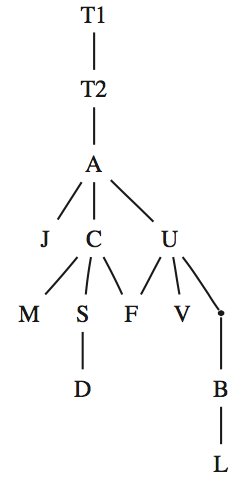
\includegraphics[scale=0.15]{figures/correct_fqp}
			\end{figure}
		\column{.32\textwidth}
			\begin{figure}
				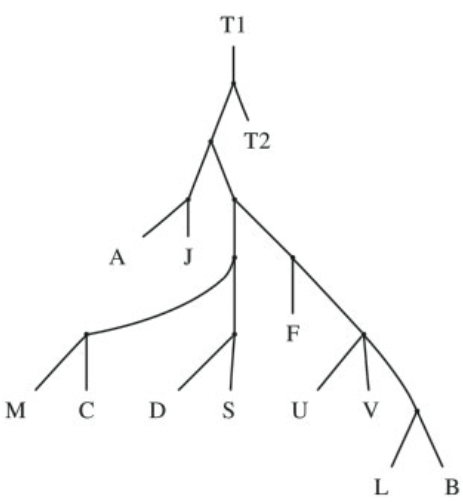
\includegraphics[scale=0.15]{figures/nj_fqp}
			\end{figure}
		\column{.32\textwidth}
		\begin{figure}
				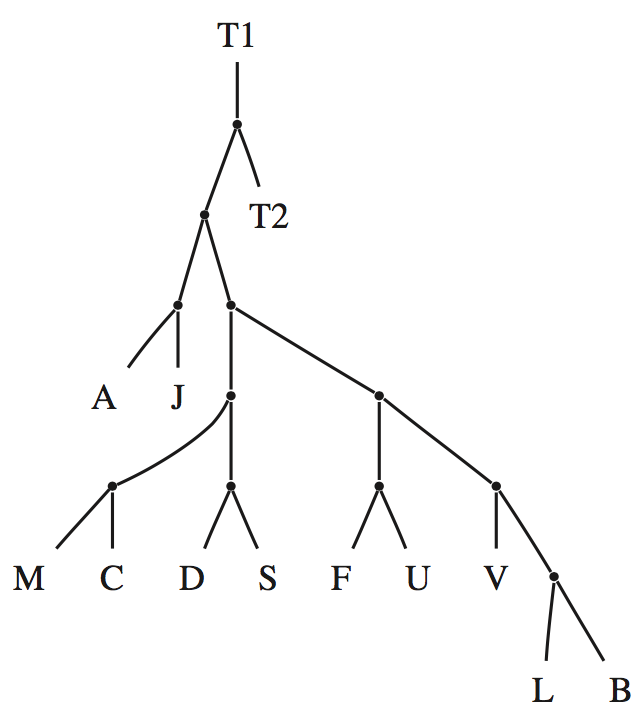
\includegraphics[scale=0.16]{figures/rhm_fqp.png}
				\caption{\tiny copied from \emph{Evaluating methods for computer-assisted stemmatology using artificial benchmark data sets}}
			\end{figure}
	\end{columns}
}

\section{Aufgabe 4}
\frame{
	\frametitle{Aufgabe 4 - Teil a}
	Die Reihenfolge in welcher die IDs der Threads ausgegeben werden ist jedes Mal unterschiedlich und ist auch nicht vorherzusagen.
}

\section{Aufgabe 5}
\frame{
	\frametitle{Aufgabe 5 -Visualisiert}
	\begin{figure}
	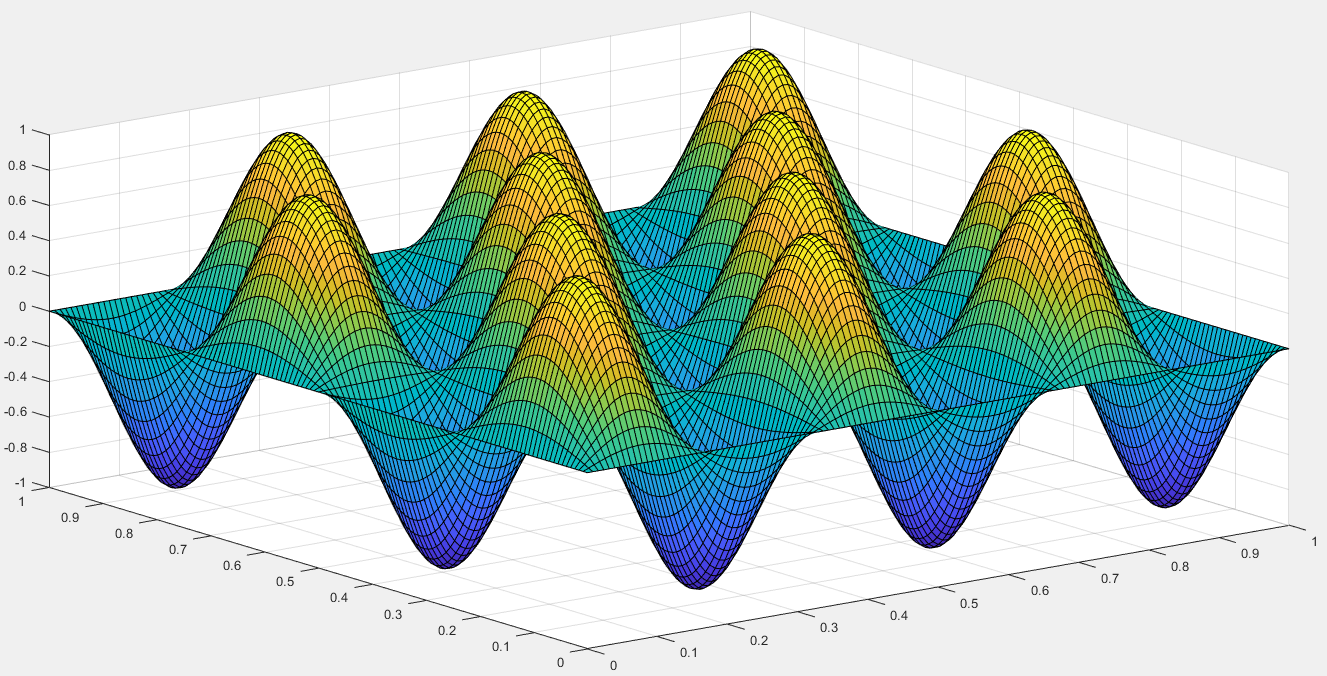
\includegraphics[width=\linewidth]{figures/A5L7M3N2.png}
		\caption{l=7; h=1/128;M=3;N=2}
	\end{figure}
}

\section{Aufgabe 6}
\frame{
	\frametitle{Aufgabe 6 - Speedup}
	\begin{tabular}{|l|l|r|r|}
		\hline
		- & Aufgabe 5(s) & Aufgabe 6(s) & Speedup\\
		\hline
		l=5; h=1/32 &   1.450 &  0.028 & 56.96 \\
		& 1.420 & 0.021 &    \\
		& 1.371 & 0.026 &    \\
		& 1.475 & 0.026 &    \\
		& 1.408 & 0.026 &   \\
		&=1.424 & =0.025  & \\
		\hline
		l=6; h=1/64 &   15.427 &  0.140 & 98.488 \\
		& 12.546 & 0.148 &    \\
		& 12.561 & 0.089 &    \\
		& 12.766 & 0.142 &    \\
		& 13.081 & 0.155 &   \\
		&=13.276 & =0.135  & \\
		\hline
		l=7; h=1/128 &  107.183 &  1.289 & 81.113 \\
		&  105.581 &  1.188 &    \\
		&  104.562 &  1.175 &    \\
		&  105.834 &  1.703 &    \\
		&  104.077 &  1.148 &   \\
		&=105.447 & =1.300  & \\
		\hline
	\end{tabular}
}
\frame{
	\frametitle{Aufgabe 6 - Visualisiert}
	\begin{figure}
	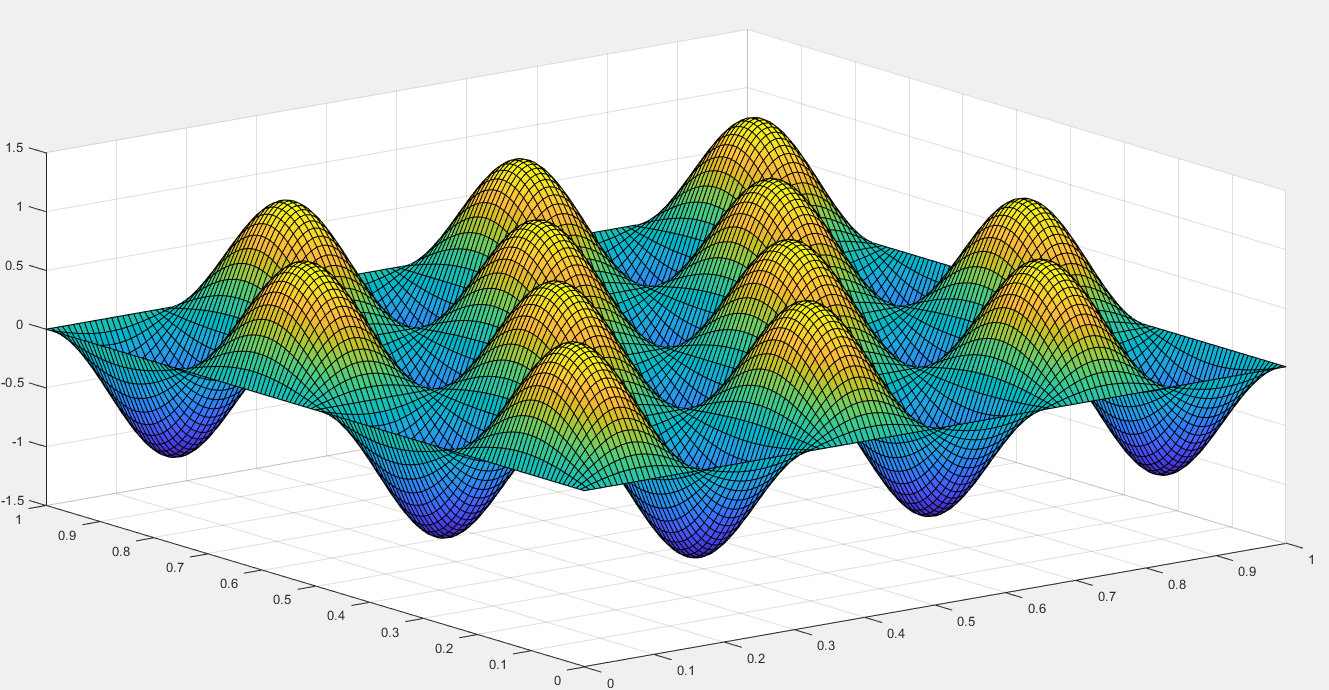
\includegraphics[width=\linewidth]{figures/A6L7M3N2.png}
		\caption{GMRES; l=7; h=1/128;M=3;N=2}
	\end{figure}
}

\section{Aufgabe 7}
\frame{
	\frametitle{Aufgabe 7}
	Die Reihenfolge in welcher die IDs der Threads ausgegeben werden ist jedes Mal unterschiedlich und ist auch nicht vorherzusagen.
}

\frame{
	\frametitle{References}
	
	\begin{itemize}
	\small
		\item Bein, Thomas. Textkritik: eine Einf"uhrung in Grundlagen germanistisch-medi"avistischer Editionswissenschaft: Lehrbuch mit "Ubungsteil. Peter Lang, 2011.
		\item Roos, Teemu, Tuomas Heikkil"a, and Petri Myllym"aki. 'A compression-based method for stemmatic analysis.' Frontiers in Artificial Intelligence and Applications 141 (2006): 805.
		\item Roos, Teemu, and Yuan Zou. 'Analysis of textual variation by latent tree structures.' Data Mining (ICDM), 2011 IEEE 11th International Conference on. IEEE, 2011.
		\item Roos, Teemu, and Tuomas Heikkil"a. 'Evaluating methods for computer-assisted stemmatology using artificial benchmark data sets.' Literary and Linguistic Computing 24.4 (2009): 417-433.
	\end{itemize}
}

\end{document}



%%% Local Variables: 
%%% mode: latex
%%% TeX-master: t
%%% End: 
